% 华电毕业论文封面 
\documentclass[UTF8,a4paper]{ctexart}
\usepackage{geometry} % 设置页边距,页面大小
\geometry{left=2.5cm,right=2.0cm,top=2.50cm,bottom=2.0cm}
\linespread{1.3}%调整行间距
\usepackage{graphicx} % 引入图片
\pagestyle{plain}    
\usepackage{setspace} %行间距
\usepackage{array} %
\usepackage{booktabs} %调整表格线与上下内容的间隔
\usepackage{multirow}
\usepackage{hyperref} %加入书签跳转
\usepackage{fontspec} %引入字体Times New Roman字体
%\setmainfont{Times New Roman}             %设置正文字体为Times New Roman
\usepackage{abstract} % 修改摘要


%\usepackage[fontset=windows]{ctex}
\usepackage{xeCJK} %调用系统中已安装的字体
\setCJKmainfont{SimSun}
\setmainfont{Times New Roman}

%% 目录格式设置
\usepackage{tocloft}      %必须这么写,否则会报错
\renewcommand{\contentsname}{\centerline{\Large{\heiti{目\quad\quad 录}}}}
%\renewcommand{\cftchapleader}{\cftdotfill{0.6}} %设置chapter条目的引导点间距
\renewcommand{\cftsecleader}{\cftdotfill{0.6}}
\renewcommand{\cftsubsecleader}{\cftdotfill{0.6}}
\renewcommand{\cftsubsubsecleader}{\cftdotfill{0.6}}
%\renewcommand{\cftchapfont}{\hts}    %设置chapter条目的字体
\renewcommand{\cftsecfont}{\heiti}    %设置section条目的字体
\renewcommand{\cftsecfont}{\Large}    %设置section条目的四号
\renewcommand{\cftsubsecfont}{\songti} %设置subsection条目的字体
\renewcommand{\cftsubsecfont}{\large} %设置subsection条目的字体
\renewcommand{\cftsubsubsecfont}{\songti} %设置subsection条目的字体
\renewcommand{\cftsubsubsecfont}{\large} %设置subsection条目的字体

% 参考文献
%\usepackage{cite}

\begin{document}
%%%%%%%%%%%%%%%%%%%%%%%%%%%
%%%%%%%%%%%%%%%%%%%%%%%%%%%


\begin{flushright}
\end{flushright}
\begin{center}
    \vskip 1.5cm
    
\includegraphics[scale=0.6]{figs/ncepu.eps}%学校图标
\end{center}
\begin{center}
    \vskip 1.5cm
    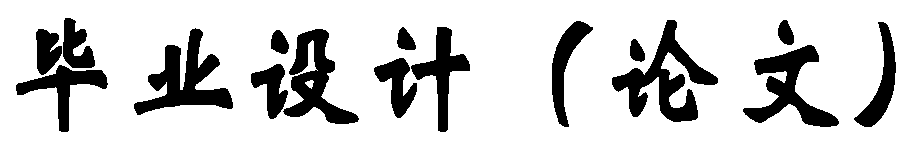
\includegraphics[scale=0.6]{figs/bthesistitle.eps}%毕业设计图标
\end{center}
\begin{center}
  \vskip 2cm
    \fontsize{15}{1} \textbf{题目} \underline{基于Qemu模拟器移植rCore操作系统的开发与实现}
	\vskip 2.5cm
\end{center}
\begin{center}
	\begin{tabular}{l}
		
		院\quad\quad 系 \underline{\qquad 控制与计算机工程学院 \quad }\\\\
		专\quad\quad 业 \underline{\qquad 计算机科学与技术 \quad\qquad}\\\\
		% \quad 代表空格,输入题目后自己调长度
		班\quad\quad 级 \underline{\qquad\quad 计算1702班 \quad\qquad\quad }\\\\
		学生姓名 \underline{\qquad\qquad 杨秉学\qquad\qquad\qquad}\\\\
		学\quad\quad 号 \underline{\qquad\quad 120171080212 \qquad\qquad }\\\\
		指导教师 \underline{\qquad\qquad\quad 琚贇\qquad\qquad\qquad }\\\\
	
	\end{tabular}
\end{center}
\begin{center}
        \vskip 2.5cm
		{2021} 年{\quad 六\quad }月{\qquad \qquad }日
		
\end{center}
\thispagestyle{empty} %去除本页页码


      
%%%%%%%%%%%%%%%%%%%%%%%%%%%%%%%%%%%%%%
%摘要
%%%%%%%%%%%%%%%%%%%%%%%%%%%%%%%%%%%%%%
%% 中文摘要
\newpage
\pagenumbering{Roman}
\renewcommand{\abstractname}{\heiti{\Large{摘\quad \quad \quad \quad 要}}}
\begin{abstract}
{\large{不要少于400字该部分内容是放置摘要信息的。该部分内容是放置摘要信息的。该部分内容是放置摘要信息的。该部分内容是放置摘要信息的。该部分内容是放置摘要信息的。}}

%\\ \hspace*{\fill} \\  %换行,用空格填充,再换行,即可实现空出一整行的效果,不需任何环境调整
\noindent %取消首航缩进
    {\large{\textbf{关键字}:RISC-V,Qemu,linux}}
\end{abstract}

%%% 英文摘要
\newpage
\renewcommand{\abstractname}{\Large \textbf{ABSTRACT}}
\begin{abstract}
{\large{This section is where the summary information is placed.This section is where the summary information is placed.This section is where the summary information is placed.}}

\noindent
\textbf{KEY WORDS:}RISC-V,Qemu,linux
\end{abstract}

%%%%%%%%%%%%%%%%%%%%%%%%%%%%%%%%%%%%%%
% 目录
%%%%%%%%%%%%%%%%%%%%%%%%%%%%%%%%%%%%%%
\newpage
\tableofcontents
\thispagestyle{empty}
%\input{part/part1}\newpage
%\input{part/part2}\newpage

\newpage
\pagenumbering{arabic}
%%定制标题样式
%%% section
\CTEXsetup[name={第,章 },format={\centering\heiti\zihao{-2}},aftername={\enspace},beforeskip={24bp},afterskip={18bp}]{section} %name选项中不要使用中文逗号 \zihao(-2)字号小二
%%% subsection
\CTEXsetup[format={\raggedright\songti\zihao{-3}},aftername={\enspace},beforeskip={24bp},afterskip={6bp}]{subsection}
%%% subsubsection
\CTEXsetup[format={\raggedright\songti\zihao{4}},aftername={\enspace},beforeskip={12bp},afterskip={6bp}]{subsubsection}

\section{背景意义}
Risc-v是一个最近流行基于RISC指令集架构,类似与软件领域开源的linux一样,Risc-V也有很多领域可以发挥作用。

\section{Risc-V模拟器原理}
\subsection{KVM \& Qemu}
首先Qemu(Quick Emulator)本身并不完全是KVM的一部分,它是一套由软件模拟实现的。

而KVM(Kernel Virtual Machine)是有两部分组成,一部分是Linux内核的KVM模块,另一块是经过简化后的Qemu。它能够让Linux主机成为一个Hypervisor(虚拟机监控器)。在支持VMX(Virtual Machine Extension)功能的x86处理器中,Linux在原有的用户模式和内核模式中新增加了客户模式,并且客户模式也拥有自己的内核模式和用户模式,虚拟机就是运行在客户模式中。三层结构如 图\ref{fig:kvm}

\begin{figure}[htbp]
  \centering %居中显示
  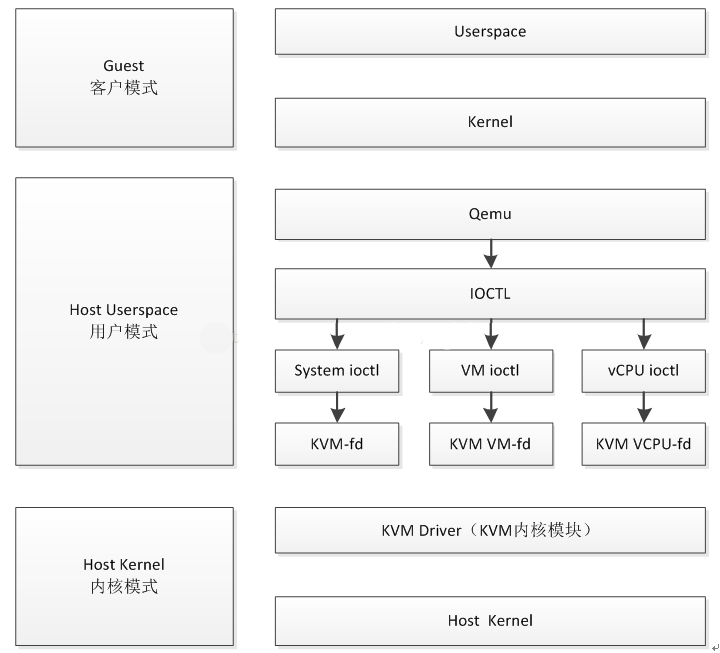
\includegraphics[width=0.6 \textwidth]{figs/KVM三种模式的层次关系.png}
  \caption{KVM三种模式的层次关系}
  \label{fig:kvm} %设置图形引用名称
\end{figure}
%『h』当前位置。将图形放置在正文文本中给出该图形环境的地方。如果本页所剩的页面不够,这一参数将不起作用。
%『t』顶部。将图形放置在页面的顶部。
%『b』底部。将图形放置在页面的底部。
%『p』浮动页。将图形放置在一只允许有浮动对象的页面上。


\subsubsection{三级标题}
正文内容
\subsection{根文件系统}
\subsubsection{Dropbear}
Dropbear是一个相对较小的SSH服务器和客户端。它运行在一个基于POSIX的各种平台,依赖zlib连接库。



\section{方案}


\section{与前人比较}

\end{document}
